% IEEE conference format. Build on Overleaf (IEEEtran is built in) or locally with:
%   pdflatex main && bibtex main && pdflatex main && pdflatex main
\documentclass[conference]{IEEEtran}
\usepackage{amsmath,amssymb}
\usepackage{graphicx}
\usepackage{booktabs}
\usepackage{url}
\usepackage[hidelinks]{hyperref}

\begin{document}

\title{Does a Learned Starting Point Make Viscosity Estimation Cheaper?\\
A Cost-Counted Study on the Burgers Equation}

% TODO: fill in team names, SRNs and e-mails.
\author{
\IEEEauthorblockN{Name 1 (SRN)}
\IEEEauthorblockA{PES University}
\and
\IEEEauthorblockN{Name 2 (SRN)}
\IEEEauthorblockA{PES University}
\and
\IEEEauthorblockN{Name 3 (SRN)}
\IEEEauthorblockA{PES University}
\and
\IEEEauthorblockN{Name 4 (SRN)}
\IEEEauthorblockA{PES University}
}

\maketitle

\begin{abstract}
We ask whether a neural network's guess of a physical parameter, used as the starting point of a
simulator-based least-squares fit, reduces the cost of the fit. The task is to recover the viscosity of the
one-dimensional Burgers equation from 4 to 16 noisy sensors with a known initial state. A two-layer
perceptron trained on 27{,}000 simulated cases predicts the logarithm of the viscosity, and a bounded
least-squares fit refines it. We count every simulator call, include the offline cost of the network, compare
against a bounded scalar search (Brent's method) and a nearest-neighbour start, and pre-registered the test
evaluation. All methods reach the same accuracy, which matches the Cram\'er--Rao bound. On the test set the
learned start saves about 2 CPU-seconds per query against a midpoint start. Against Brent's search it
saves 0.8--1.1 CPU-seconds at one stopping tolerance and nothing measurable at a tighter one, so the
pre-registered criterion is not met; matched on typical precision the gain is about 1.2$\times$, against a
2$\times$ target. Using the guess as a search bracket for Brent instead saves 8--10\% at Brent's own precision,
a follow-up designed after the main test. The saving of the least-squares route disappears for starting states
and sensor patterns not seen in training.
\end{abstract}

\begin{IEEEkeywords}
learned initialization, inverse problems, Burgers equation, parameter estimation, amortized optimization
\end{IEEEkeywords}

% Sections I-V. Every number here is taken from a committed file; the source is named in a comment.

\section{Introduction}
Estimating a physical parameter from a few sensor readings usually means fitting a simulator to the data:
an optimiser proposes a parameter value, the simulator is run, and the mismatch with the readings decides the
next proposal. When each run is expensive, the number of runs is the cost. A common idea is to train a neural
network on simulated examples so that it predicts the parameter directly, and to use that prediction as the
starting point of the fit. The fit then keeps its accuracy and, one hopes, needs fewer runs.

We test this idea on a deliberately small problem where every part can be checked: recovering the viscosity
$\nu$ of the one-dimensional viscous Burgers equation from 4, 8 or 16 sensors read at four times, with a
known initial state and 0\%, 1\% or 5\% noise. A two-layer perceptron predicts $\log\nu$; a bounded
least-squares fit refines it. Our project proposal set a target: the learned start should halve the median
online cost at no loss of accuracy. We state that as a hypothesis and test it.

Three choices shape the study. First, the comparison includes a direct bounded scalar search (Brent's method),
which needs no starting point at all, and a nearest-neighbour start; a learned start that only beats a poor
cold start has shown little. Second, cost counts every simulator call, including those used for
finite-difference derivatives, and the offline cost of the network (data generation, tuning, training) is
divided by the saving per query to give a break-even number of queries. Third, the test-set evaluation was
written down and committed before the test set was used, and it is reported whatever the outcome.

The outcome is mostly negative. The learned start makes the least-squares fit cheaper than a midpoint start
in every setting we ran. Against Brent's search, it is cheaper at one stopping tolerance and not at a tighter
one, and the 2$\times$ target is not met. The remaining sections show why: the estimates already reach the
Cram\'er--Rao bound, so accuracy cannot separate the methods, and a one-dimensional search needs so few
simulator runs that little is left to save.

\section{Related Work}
\textbf{Learned warm starts.} Sambharya et al.~\cite{sambharya2024} train a network that maps the parameters
of a convex problem to a warm start for a fixed-point solver, and compare it with a cold start and a
nearest-neighbour warm start; they report iterations and solve times, and state training time separately
without setting it against the savings. Zhou et al.~\cite{zhou2023} predict the shape of a scattering
obstacle with a convolutional network and refine it by Gauss--Newton; their aim is to avoid local minima at
high frequency, they report running time per obstacle, and training time is excluded from that comparison.
Borisyak et al.~\cite{borisyak2023} predict the parameters of ODE growth models and optionally refine them by
gradient-based fitting. Oh et al.~\cite{oh2026} warm-start Newton solvers for nonlinear PDEs with a neural
operator and show that a low prediction error does not by itself give a usable start. Amos~\cite{amos2023}
surveys this family as amortised optimisation; in his terms our method is semi-amortised and trained by
regression.

\textbf{Amortised and surrogate-based parameter estimation.} Simulation-based inference replaces the
optimiser by a network trained on simulations~\cite{cranmer2020}; Tatsuoka et al.~\cite{tatsuoka2025} do so
with two fidelity levels to limit expensive forward runs. Roy Sarkar et al.~\cite{roysarkar2024} identify PDE
parameters from sparse, noisy data, Burgers among the examples, with a pretrained operator network in place
of the simulator, and Long et al.~\cite{long2025} train a recurrent network together with a numerical scheme
for each problem. We keep the simulator in the loop and learn only the starting point.

\textbf{Sensors and identifiability.} Neitzel et al.~\cite{neitzel2019} choose sensor locations by the
covariance of the least-squares estimator. We use the same Fisher-information view, not to place sensors but
to check whether our estimates use all the information the given sensors carry.

\textbf{Position of this work.} The mechanism is established; we do not claim it. What the two closest
works~\cite{sambharya2024,zhou2023} leave open, and what we measure on one small problem, is the comparison
against a direct scalar search, the break-even count once offline cost is included, and the dependence of the
saving on the stopping tolerance.

\section{Problem Setup}
\subsection{Equation and simulator}
We use the Burgers equation in the PDEBench convention~\cite{takamoto2022}, % configs/simulator_v1.json
\begin{equation}
u_t + \left(\tfrac{1}{2}u^2\right)_x = \frac{\nu}{\pi}\,u_{xx}, \qquad x\in[0,1)\ \text{periodic},
\end{equation}
with $\nu\in[0.01,0.1]$ and the initial state
$u_0(x)=\sum_{k=1}^{3} a_k \sin(2\pi k x+\phi_k)$, $a_k\sim U(0,1)$, $\phi_k\sim U(0,2\pi)$. The amplitudes and
phases are known to every method; only $\nu$ is unknown. The solver is our own NumPy implementation of the
finite-volume scheme used by PDEBench (MUSCL reconstruction with its limiter, Rusanov flux, central
diffusive flux, two-stage midpoint time stepping, CFL 0.25) on 256 cells in double precision. No PDEBench
code is included.

The solver passes eleven tests, % tests/test_simulator.py
among them convergence to the exact Cole--Hopf solution, the small-amplitude heat limit with diffusivity
$\nu/\pi$, mass conservation and periodic shift invariance. Its cost depends on $\nu$ because the explicit
diffusion step limits the time step: one run to $t=1$ takes 1{,}686 steps at $\nu=0.01$ and 16{,}692 at
$\nu=0.1$. % RESEARCH_LOG.md, "Cost observation"
A method's cost therefore depends on which values of $\nu$ it tries, not only on how many.

\subsection{Observations}
Sixteen sensor slots sit at $x_s=(s+0.5)/16$ and are read at $t\in\{0.25,0.5,0.75,1\}$. A case uses 16, 8 or
4 of them (every slot, every second, every fourth). Gaussian noise of standard deviation
$\sigma=\ell\cdot\mathrm{RMS}$ is added, where $\ell\in\{0,0.01,0.05\}$ and RMS is taken over the clean
$16\times4$ readings of that trajectory. % blinit/data.py make_observations
Each trajectory thus gives nine cases (three sensor counts $\times$ three noise levels).

\subsection{Data}
No public dataset is used; all data are generated by the repository's solver from versioned configuration
files and regenerate identically. % configs/phaseB_v2.json, data/phaseB_v2/integrity.json
There are 3{,}000 training, 50 validation and 50 test trajectories (27{,}000 / 450 / 450 cases), with $\nu$
drawn log-uniformly. Splits are made by the seed of the initial state, so all noise and sensor variants of a
trajectory stay in one split. Nine automated checks run at build time, covering seed overlap between splits,
normalisation statistics taken from training data only, and the mapping from readings to sensor positions.

\section{Methods}
All methods estimate $\theta=\log\nu$ within $[\log 0.01,\log 0.1]$ by minimising
$J(\theta)=\tfrac12\lVert f(\theta)-y\rVert^2$ over the available readings, where $f$ is the simulator
followed by interpolation to the sensors. They share one problem object that counts every simulator call.
% blinit/inverse.py

\textbf{Brent.} Bounded scalar minimisation of $J$ (SciPy \texttt{minimize\_scalar}, method
\texttt{bounded}) with absolute tolerance \texttt{xatol} on $\theta$. It needs no starting point.

\textbf{Start + LSQ.} A starting value $\theta_0$ followed by bounded least squares (SciPy
\texttt{least\_squares}, trust-region reflective, two-point finite differences with relative step
$10^{-6}$, tolerance \texttt{xtol}). Four starts are compared:
\emph{midpoint} of the interval; \emph{grid}, the best of five log-spaced values (five extra simulator runs,
counted); \emph{kNN}, the inverse-distance-weighted mean of the $k$ nearest training cases with the same
sensor pattern; and \emph{MLP}.

\textbf{MLP.} A perceptron with two hidden layers of 64 ReLU units (scikit-learn \texttt{MLPRegressor},
Adam, batch size 64) maps 134 inputs to $\log\nu$: the 64 standardised readings with missing ones set to
zero, 64 availability flags, and the six numbers $a_k\cos\phi_k$, $a_k\sin\phi_k$. % configs/phaseC_v2.json
Training stops early on the validation loss. Four settings of learning rate and weight decay were tried and
the one with the lowest validation loss kept; three seeds were then trained. % models/phaseC_v2/tuning.json
kNN's $k$ and feature weight were chosen on validation as well. The test split was not loaded during any of
this.

\textbf{Cost.} The cost of a query is its number of solver steps times 144.3\,\textmu s, the median time per
step measured in sequential runs. % RESEARCH_LOG.md, Phase A run 2
We use steps rather than wall-clock time because experiments ran on parallel workers of a laptop whose
timings were not clean. The offline cost of the MLP is the wall time of training-data generation multiplied
by the number of workers (an upper bound), plus tuning and training. % blinit/experiments/analyze_d.py
The break-even count is this offline cost divided by the mean saving per query against the cheapest
classical method, with the MLP's inference time subtracted from the saving.

\section{Evaluation Protocol}
\textbf{Tolerances.} Stopping tolerances were fixed on development data: Brent \texttt{xatol} $10^{-3}$ and
LSQ \texttt{xtol} $10^{-3}$ (primary). Because the LSQ rule can stop looser than Brent in the worst case, a
second setting with LSQ \texttt{xtol} $10^{-4}$ (accuracy-matched) was added before testing.

\textbf{Pre-registration.} Before the test split was used, a document committed to the
repository % docs/preregistration_pilot_test.md
fixed the models, the methods, both tolerance settings, the cost metric, the statistic (median paired
difference in CPU-seconds between a learned method and Brent on the same case, with a 95\% bootstrap interval
that resamples trajectories), and the rule for success: the saving counts as positive only if the interval
excludes zero under both tolerance settings for at least two of the three MLP seeds. The 2$\times$ target is
judged on the ratio of median costs. The test split was evaluated once per setting and nothing was changed
afterwards. The robustness sets of Section~\ref{sec:robust} were pre-registered in the same way before they
were generated. % docs/preregistration_phaseF.md

\textbf{What validation was used for.} Early stopping, the choice among four MLP settings, the kNN settings,
the tolerance curves of Section~\ref{sec:tol} and the ablations. Validation numbers are labelled as such.

% Sections VI-IX. Every number is taken from a committed file; the source is named in a comment.

\section{Results}

\subsection{Development findings: how much can a starting point save?}
% results/phaseA/summary.json, results/phaseA_noise/, results/phaseA/init_sweep.csv; RESEARCH_LOG.md Session 1-2
On 20 noise-free development problems with 16 sensors, every method recovered $\nu$ (worst relative error
$1.2\times10^{-5}$), and the misfit $J$ had a single minimum in all of them. With 1\% and 5\% noise and 4 or
8 sensors, objective scans of 160 problem--condition pairs again showed no second minimum, and every method
reached the same optimum. Hard cases are therefore hard because the data carry little information, not
because an optimiser fails. Fig.~\ref{fig:objective} shows typical misfit curves.

This bounds what any starting point can do. A start placed at the true value (a diagnostic that reads the
truth, never a method) still needed about 6 simulator runs to stop under noise, against 9--10 for Brent.
No initialiser can therefore beat Brent by much more than 1.5$\times$ in runs on this problem. A start
within 1\% of the truth saved about 3 runs, one within 10\% about 1. The MLP's validation error is 8--12\%
(median over three seeds), so the expected saving was about one run per query before any test was run.
% models/phaseC_v2/summary.json

\begin{figure}[t]
\centering
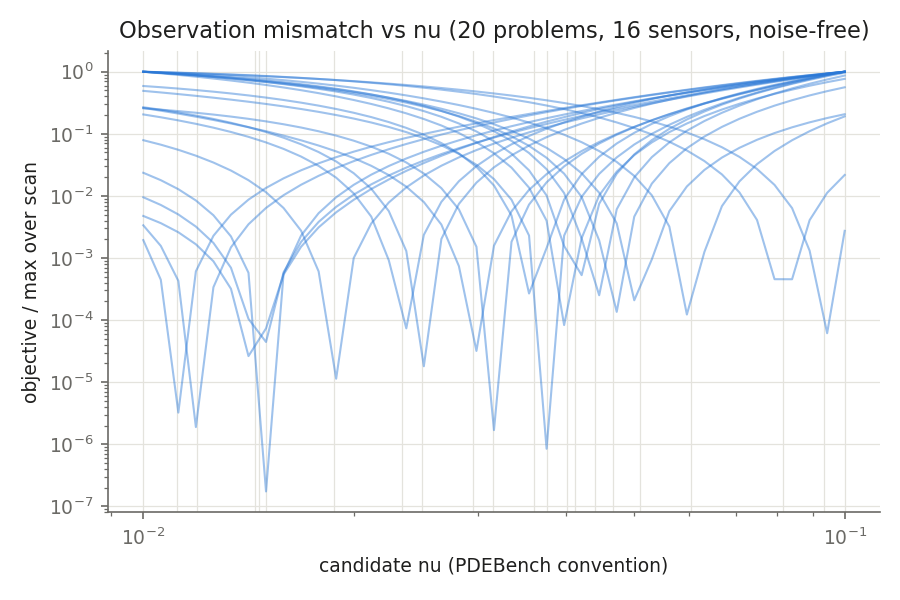
\includegraphics[width=\columnwidth]{figures/objective_curves.png}
\caption{Misfit $J$ against $\nu$ for development problems: one minimum in every case.
Source: \texttt{results/phaseA/figures}.}
\label{fig:objective}
\end{figure}

\subsection{Pre-registered test: learned start versus Brent}
% results/phaseD_v1_3seeds_test/analysis.json, results/phaseD_v1_tightlsq_3seeds_test/analysis.json
Table~\ref{tab:test} gives the 450 test cases at the primary tolerance. All methods reach the same accuracy
(median relative error 0.22\%, 90th percentile 2.6\%), with no simulator failures, so the comparison is about
cost alone. The MLP start needs the fewest runs (median 8) and the lowest mean cost.

\begin{table}[t]
\caption{Pilot test, 450 cases, primary tolerance. Error: relative error in $\nu$.}
\label{tab:test}
\centering\small
\begin{tabular}{@{}lccc@{}}
\toprule
Method & Error med / p90 & Runs med & CPU-s mean / med \\
\midrule
Brent & 0.22\% / 2.6\% & 9 & 9.01 / 8.12 \\
Midpoint + LSQ & 0.22\% / 2.6\% & 10 & 11.06 / 7.37 \\
Grid + LSQ & 0.22\% / 2.6\% & 12 & 12.79 / 11.75 \\
kNN + LSQ & 0.22\% / 2.6\% & 8 & 9.27 / 7.65 \\
MLP + LSQ (seed 0) & 0.22\% / 2.6\% & 8 & 8.20 / 6.75 \\
\bottomrule
\end{tabular}
\end{table}

Fig.~\ref{fig:paired} shows the pre-registered statistic. At the primary tolerance all three seeds are
cheaper than Brent, by a median of 0.80 to 1.07 CPU-seconds per query, with intervals that exclude zero.
At the accuracy-matched tolerance the median differences shrink to $-0.03$ to $-0.12$ and every interval
includes zero; the mean difference turns positive ($+0.21$ to $+0.56$), meaning the MLP route is slightly
costlier on average. The success rule required an interval excluding zero under both settings for two of
three seeds; it held for three seeds under one setting and none under the other.
\textbf{The pre-registered result is therefore not positive.} The ratio of median costs, Brent over MLP, is
1.13--1.22 at the primary tolerance and 1.01--1.05 at the matched one, so \textbf{the 2$\times$ target is not
met}. Against the midpoint start, the MLP start saves 1.9--2.5 CPU-seconds per query in both settings, with
every interval below zero: the learned start does help the least-squares fit, just not enough to overtake
Brent. kNN is no cheaper than Brent at the primary tolerance and costlier at the matched one.

Counting offline cost (2{,}254 CPU-seconds for data generation, tuning and training of seed 0), the break-even
point against Brent is 2{,}790, 2{,}625 and 4{,}455 queries for the three seeds at the primary tolerance. At
the matched tolerance the mean saving is not positive, so there is no finite break-even.

\begin{figure}[t]
\centering
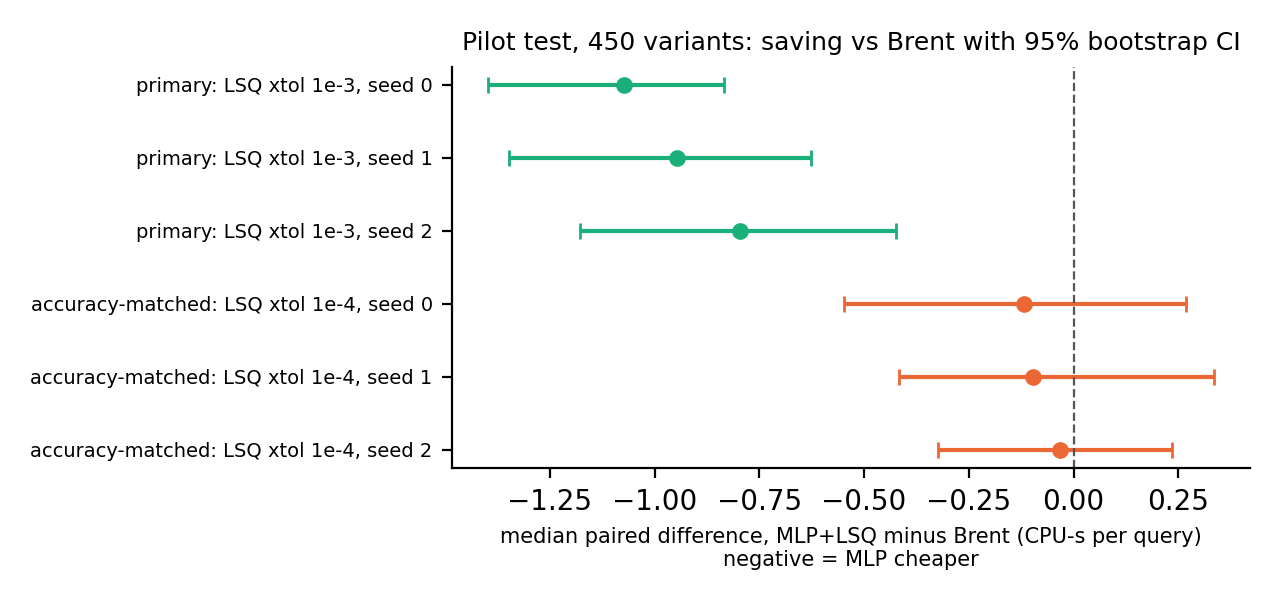
\includegraphics[width=\columnwidth]{figures/test_paired.png}
\caption{Pre-registered statistic on the pilot test: median paired cost difference, MLP+LSQ minus Brent,
with 95\% bootstrap intervals over trajectories. Source: \texttt{results/phaseD\_v1*\_3seeds\_test}.}
\label{fig:paired}
\end{figure}

\subsection{Why the saving depends on the tolerance}\label{sec:tol}
% results/phaseF_tolerance/{curves.csv,matched.json}
The two tolerance settings are not exactly matched in precision, so on validation we ran each method at three
or four tolerances and measured precision against a very tight Brent solution ($\texttt{xatol}=10^{-7}$) for
each case (Fig.~\ref{fig:tol}). Matched on the 90th-percentile precision, the MLP route is cheaper than Brent
by a factor of 1.17--1.22 in mean cost across precisions from $10^{-3}$ to $3\times10^{-5}$. Matched on the
worst case, the factor is 1.05 at $10^{-3}$ and 0.95 at $3\times10^{-4}$.

The worst case is where least squares is weak. Each tenfold tightening of Brent's tolerance cuts its largest
error about tenfold. From the MLP start the largest error falls only from $5.0\times10^{-4}$ to
$2.7\times10^{-4}$ between \texttt{xtol} $10^{-4}$ and $10^{-5}$, and from the midpoint start one case stays
at $1.1\times10^{-3}$ at both. The primary setting looked favourable because least squares stops early on a
few hard cases; once those are held to Brent's precision the saving goes. These curves use validation data,
on which the MLP was early-stopped and tuned, so they favour the MLP if anything.

\begin{figure}[t]
\centering
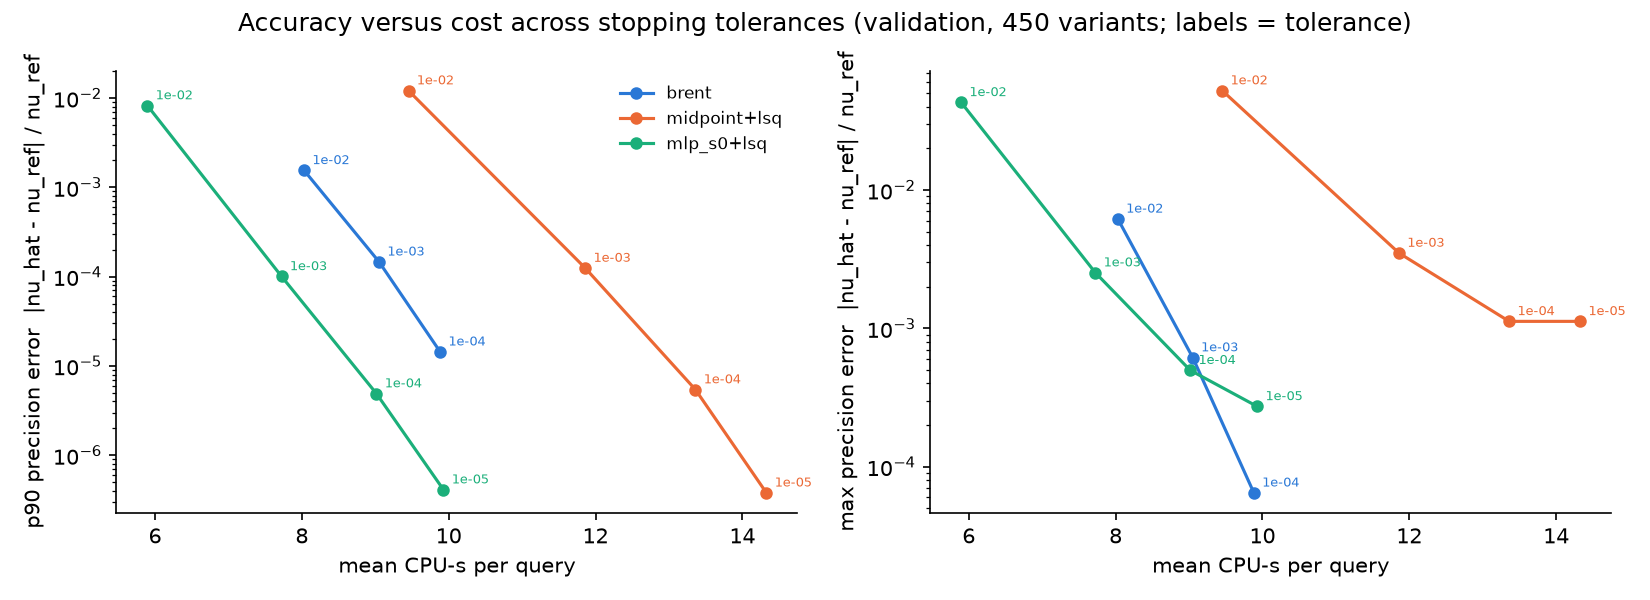
\includegraphics[width=\columnwidth]{figures/tolerance_curves.png}
\caption{Cost against precision across stopping tolerances (validation). Left: 90th percentile; right:
worst case. Source: \texttt{results/phaseF\_tolerance}.}
\label{fig:tol}
\end{figure}

\subsection{Follow-up: Brent inside a learned bracket}\label{sec:bracket}
% results/followup_bracket_val/analysis.json, results/followup_bracket_w0.5_3seeds_test/analysis.json;
% docs/preregistration_followup_bracket.md; RESEARCH_LOG.md Session 3
If least squares loses its advantage in the worst case, the learned guess can be given to Brent instead: Brent
searches $[\hat\theta_{\mathrm{MLP}}-w,\ \hat\theta_{\mathrm{MLP}}+w]$ with its own tolerance, so precision is
matched by construction, and if the estimate lands on an interior edge of the bracket, Brent is rerun on the
full interval with all runs counted. The half-width $w=0.5$ (in $\log\nu$) was chosen on validation from
$\{0.1,0.2,0.3,0.5\}$; it is the edge of that grid. This variant was designed after the main test result was
known and was then evaluated on the same 450 test cases under its own pre-registration, so it is weaker
evidence than the main test.

On test it falls back to the full interval in 1.6--2.7\% of cases, matches Brent's accuracy (its estimates
differ from Brent's by at most $3.3\times10^{-4}$ relative), and is cheaper than plain Brent for all three
seeds: median paired difference $-0.96$ to $-1.11$ CPU-seconds, every interval below zero, mean difference
$-0.69$ to $-0.92$ (an 8--10\% mean saving). The ratio of median costs is 1.04--1.11, and break-even comes
after about 2{,}400--3{,}300 queries. This is the one setting where a learned guess gave a saving over
Brent at matched precision; it is small, and it needs confirmation on fresh trajectories.

\subsection{The estimates reach the Cram\'er--Rao bound}
% results/phaseF_crb/table_test.json, table_val.json
For readings $y=f(\theta)+\varepsilon$ with Gaussian noise of standard deviation $\sigma$, the Fisher
information about $\theta=\log\nu$ is $I(\theta)=\sigma^{-2}\sum_i (\partial f_i/\partial\theta)^2$ over the
available readings, and an unbiased estimator has $\mathrm{Var}(\hat\theta)\ge 1/I(\theta)$. We computed the
derivatives by central differences in $\theta$ (step $10^{-3}$; a step of $10^{-4}$ changes them by under 1\%)
and formed $z=(\hat\theta-\theta)/\sqrt{1/I}$ for the 300 noisy test cases. If the estimator attains the
bound, $z$ has unit spread. On test, the spread of $z$ is 0.947 for Brent and 0.944 for the MLP route (0.965
and 0.966 on validation), the mean is $-0.002$, and 3.3--3.7\% of cases have $|z|>2$, against 5\% for a unit
normal (Fig.~\ref{fig:crb}). \textbf{Both methods extract all the information the sensors carry.} Accuracy
cannot separate the methods, and no method could be more accurate on these data; only cost is left to
compare. The bound assumes an unbiased estimator and ignores the bounds on $\nu$, which can let estimates
near the bounds beat it slightly.

\begin{figure}[t]
\centering
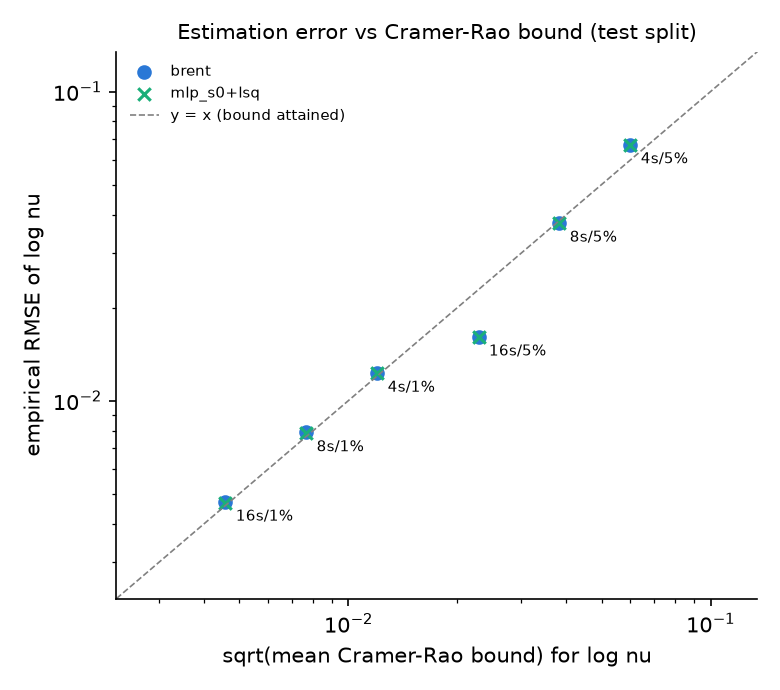
\includegraphics[width=0.85\columnwidth]{figures/crb_test.png}
\caption{Empirical error of $\log\nu$ against the Cram\'er--Rao bound, per sensor/noise condition (test).
Points on the line attain the bound. Source: \texttt{results/phaseF\_crb}.}
\label{fig:crb}
\end{figure}

\subsection{Robustness to shifted data}\label{sec:robust}
% results/phaseD_v1_3seeds_test_phaseF_{highfreq,finegrid,unseenmask}/analysis.json; docs/preregistration_phaseF.md
Three further test sets of 50 new trajectories each were generated after their analysis was pre-registered;
the models were not changed. Fig.~\ref{fig:robust} summarises them.

\emph{Higher-frequency starting states} (sine modes 2--4 instead of 1--3). The MLP's own error triples, to a
median of 28--33\% (against 9--14\% on the pilot test). Refinement still reaches the same accuracy as Brent,
but the saving disappears: the median difference against Brent is $+0.07$ to $+0.38$ CPU-seconds with every
interval including zero.

\emph{Data from a finer grid} (simulated on 1{,}024 cells, inverted on 256). This mimics data that do not come
from the model used for fitting. Every method's error rises to a median of 0.62\%, a model error no method
removes. The MLP's own error is unchanged (9--11\%) and the saving against Brent holds: $-1.19$ to $-1.41$
CPU-seconds, every interval below zero, break-even 1{,}567--2{,}606 queries.

\emph{Sensor patterns not seen in training.} On four new patterns the MLP alone has a median error of
49--61\%, no better than guessing the midpoint (57\% on validation), and the saving against Brent is gone
(median difference $+0.40$ to $+0.70$; intervals include zero). On the two patterns seen in training,
evaluated on the same trajectories, the saving remains ($-0.91$ to $-1.17$, every interval below zero).
Even the gain over a midpoint start shrinks there, to a median of 0.41--0.70 CPU-seconds, with intervals that
touch zero for some seeds. kNN, which falls back to all-sensor neighbours and compares only the available
readings, gives a better start on unseen patterns (22--31\%) but is still costlier than Brent.

The pattern is the one stated before the runs: when the inputs differ from training, the network's start
gets worse and the least-squares fit absorbs it, at the price of the saving.

\begin{figure*}[t]
\centering
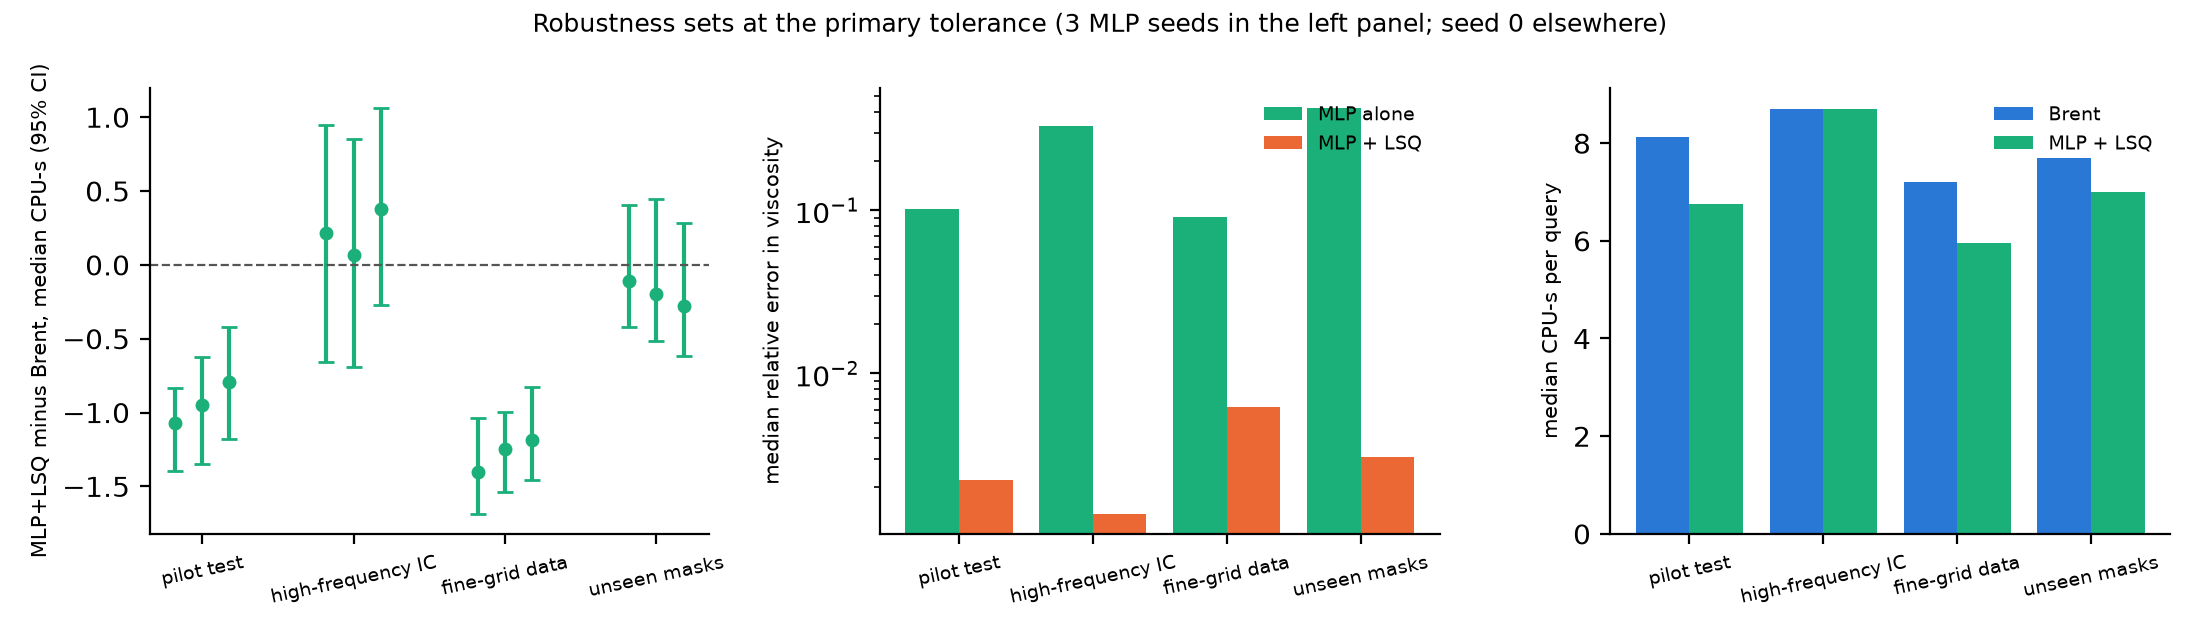
\includegraphics[width=0.9\textwidth]{figures/robustness.png}
\caption{Robustness sets at the primary tolerance. Left: MLP+LSQ minus Brent, three seeds, 95\% intervals.
Middle: error of the MLP alone and after refinement. Right: median cost. Source:
\texttt{results/phaseD\_v1\_3seeds\_test\_phaseF\_*}.}
\label{fig:robust}
\end{figure*}

\subsection{Ablations}
% results/phaseF_ablations/ablations.md (validation)
\emph{Network alone versus network plus refinement.} The MLP alone has a median error of 8.2\% (90th
percentile 33\%); after refinement it is 0.245\%. The network alone is about 33 times less accurate than the
data allow, so refinement cannot be dropped.

\emph{Training with missing sensors.} Our MLP trains on all three sensor counts. Trained on 16-sensor cases
only, its error at 4 sensors is 55\% (against 10--13\%) and at 8 sensors 36\% (against 9--11\%); at 16
sensors the two are equal. Together with the unseen-pattern result, this says the augmentation helps exactly
for the patterns it contains.

\emph{Known starting state as input.} Setting the six starting-state inputs to zero raises the error at 4
sensors from 10--13\% to 14--17\% and changes nothing outside the seed spread at 8 or 16 sensors. The network
uses the starting state only when the readings are few.

\section{Limitations}
The study covers one equation, one unknown scalar, and synthetic data from our own solver; the fine-grid set
is the only test of model mismatch. The competitor that matters, a one-dimensional bounded search, is
unusually strong because the misfit has a single minimum; with several unknowns or several minima a learned
start may matter more. Cost is counted in solver steps times a fixed time per step, measured once on one
laptop, because parallel wall-clock times were not clean; network inference time is included but is
negligible. Test sets have 50 trajectories each, so intervals are wide. The offline cost uses generation wall
time multiplied by worker count, an upper bound. Validation data were used both for early stopping and for
the tolerance curves and ablations, which favours the learned method in those analyses. The learned-bracket
follow-up (Section~\ref{sec:bracket}) was designed after the main test result and reuses the same test cases;
it was not run on the robustness sets. An optional larger
test set for the main claim (200 trajectories) was planned and not run.

\section{Conclusion}
A small network's guess makes a least-squares fit of Burgers viscosity cheaper than starting from the middle
of the range, by about 2 CPU-seconds per query on the test set; on sensor patterns not seen in training that
gain shrinks to about 0.5 and is not always distinguishable from zero. It does not make the fit reliably
cheaper than Brent's bounded search, which needs no guess: at equal typical precision it saves about
1.2$\times$, at equal worst-case precision about nothing, and the pre-registered test was not positive.
Handing the guess to Brent as a search bracket instead does save 8--10\% at Brent's own precision, a small
gain found after the main test and not yet confirmed on fresh data. Where
it does save, it pays back its offline cost after roughly 1{,}600--4{,}500 queries. The saving vanishes when
the starting states or sensor patterns differ from training. Since both methods already reach the
Cram\'er--Rao bound, the only room left is cost, and on a single-minimum scalar problem a direct search
leaves little of it. We did not observe the 2$\times$ speed-up the proposal hypothesised.

\section*{Data and Code Availability}
No public dataset is used. All data are generated by the solver in the repository from versioned
configuration files (\texttt{configs/phaseB\_v2.json} and \texttt{configs/phaseF\_*.json}) and regenerate
identically with one command each. The numerical scheme follows PDEBench~\cite{takamoto2022}, whose released
Burgers data we did not use because they fix one viscosity per file and use different starting states.
Code, configurations, trained models, result files and a log of every run:
\url{https://github.com/minkysponge-wq/Afml-Mini-project}.

\section*{Acknowledgment}
The numerical scheme of our solver follows the Burgers data generator of PDEBench, software developed by NEC
Laboratories Europe; our solver is an independent re-implementation and contains none of its code.


\bibliographystyle{IEEEtran}
\bibliography{refs}

\end{document}
